\documentclass[10pt,a4paper]{article}
\usepackage[margin=2.4cm]{geometry}
\usepackage{amsmath}
\usepackage{booktabs}
\usepackage{graphicx}
\usepackage{caption}
\usepackage{subcaption}
\usepackage{microtype}
\usepackage{listings}
\usepackage{xcolor}
\usepackage[numbers,sort&compress]{natbib}
\usepackage[colorlinks=true,linkcolor=blue!55!black,citecolor=blue!55!black,urlcolor=blue!55!black]{hyperref}
\hypersetup{pdftitle={To Buffer or Not to Buffer: An Empirical Study of Channel Buffer Capacity in Go, with a Measurement-Driven Auto-Tuner},
            pdfauthor={Jatin J.},
            pdfsubject={Empirical study of Go channel buffer capacity and a measurement-driven auto-tuner}}

\lstset{language=Go,basicstyle=\ttfamily\footnotesize,numbers=left,numberstyle=\tiny\color{gray},
        frame=single,framerule=0.3pt,columns=fullflexible}

\title{To Buffer or Not to Buffer:\\ An Empirical Study of Channel Buffer Capacity in Go,\\
       with a Measurement-Driven Auto-Tuner}
\author{Jatin J.\thanks{All the code, raw data, and this document are in the
project directory \texttt{research-paper}; the harness, library, and analysis
scripts are listed in Appendix~\ref{app:repro}.}}
\date{October 27, 2026}

\begin{document}
\maketitle

\begin{abstract}
Channels are Go's idiomatic mechanism for moving values between different
goroutines, and the buffer capacity supplied at construction is the one
quantity a programmer must choose for them. That choice is presently folklore:
advice ranges from ``always use an unbuffered channel'' to ``make it big, just
in case,'' and the two camps cannot both be right. We present, to our
knowledge, the first systematic characterization of how the capacity affects a
shared channel's throughput and latency distribution. The harness routes
timestamped messages through one shared channel under four sender/receiver
topologies, eleven capacities from unbuffered to 512, and both value and
pointer channel types, with five repetitions per configuration on a 16-core
Linux machine running Go 1.26. Throughput saturates quick: small capacities
capture at least 99\% of the best observed throughput (at capacity 32--64
depending on topology), and capacities beyond that point buy nothing
measurable. Unbuffered Handshakes costs 40--92\% of the best capacity's
throughput, with the largest losses where senders outpace receivers. The
latency tail behaves quite differently from the head: p99 latency grows
roughly linearly with capacity once senders outpace receivers, so an oversized
buffer converts spare capacity directly into queueing delay. Based on the
findings we implement \texttt{autobuf}, a small library that treats capacity
as a hyperparameter: it probes the caller's real pipeline once per candidate
capacity, scores each probe by measured throughput, and returns the winner.
Across 40 independent invocations spanning 4 topologies, the tuner's choice
achieves 99.9--102.1\% of the best candidate capacity's throughput under
identical measuring conditions. We clean the measurements into a short
decision rule for practitioners and release the harness, library, and raw data
for replication.
\end{abstract}

\section{Introduction}
\label{sec:intro}

Go's concurrency model rests on two primitives which are goroutines and
channels. Goroutines are cheap user-scheduled threads; channels are typed
conduits through which goroutines exchange values. These both come from the
communicating-sequential-processes tradition \cite{hoare}, which the Go team
cites as the design basis for the language's concurrency
\cite{pikepatterns,pikeconc}. Since Go 1.0 the idiomatic way to connect
concurrent components has been to connect them with one channel, and the one
decision a programmer makes at channel creation time is the buffer capacity:
\texttt{make(chan T, n)}.

The second argument is, in effect, the hyperparameter. With capacity zero the
channel becomes a rendezvous point: every send blocks until the receiver is
ready, which forces strict lock-step synchronization. Once a positive capacity
is set, the sender may deposit its value and move on, decoupling the two
goroutines in time. Between these extremes lies a range of choices whose
consequences are hard to reason about from the language specification alone,
because they depend on scheduler behavior, core counts, and the arrival pattern
of real work.

Practice does not help much in this case. In tutorials and code review comments
one finds advice in both these directions. Some programmers insist on
unbuffered channels so that hand-offs are explicit and backpressure is
immediate; others sprinkle buffers of around eight, sixteen, or a hundred to
``avoid contention.'' Signal semaphores conventionally use a capacity of one.
Pipeline stages often get some generous buffer ``in case of bursts.'' None of
this is tested systematically anywhere we can find, and the camps contradict
one another: an unbuffered channel and a capacity-512 channel cannot both be
optimal.

The cost of a wrong choice is real but not even. Our measurements show the two
error modes are qualitatively different. Choosing zero when a small buffer would
do allows throughput on the table, because every hand-off degenerates into a
goroutine park and wake. Choosing large when small would do doesn't raise
throughput at all, but silently stretches the latency tail, since buffered
messages accumulate and wait. In a service where a goroutine sits behind
that channel, capacity is a p99 setting as much as the throughput one.

This paper answers three questions:
\begin{description}
  \item[Q1] How does capacity affect throughput, as the function of the
        sender/receiver topology around the channel?
  \item[Q2] How does the capacity affect the latency distribution of individual
        messages, particularly the tail?
  \item[Q3] Can a program choose a good capacity for itself, at start-up,
        without a human doing benchmarking by their hand?
\end{description}

Our approach is very direct. We built a small harness that routes realistic
messages through a single shared channel, stamps each one at dispatch and at
receipt, and reconstructs both aggregate throughput and per-message latency
percentiles. We then went through capacities from zero to 512 under four
sender/receiver topologies, repeated each configuration five times, and
repeated the sweep for pointer-typed channels where each message is a separate
heap allocation. Finally we wrote the \texttt{autobuf} library, which applies
the same measurement idea to the programmer's actual pipeline: it builds each
candidate capacity shortly, scores each probe, and returns the winner.

The contributions are:
\begin{itemize}
  \item \textbf{C1 (characterization).} A systematic sweep of capacity
        (11 values), topology (4 topologies), channel type (value vs.\ pointer),
        and repetition ($n=5$), on one 16-core machine with Go 1.26 under
        Linux. The harness, the full CSV output, and the analysis scripts
        accompany this paper.
  \item \textbf{C2 (findings).} Five findings, summarized in
        Section~\ref{sec:results} and quantified in
        Tables~\ref{tab:sweep}--\ref{tab:tuner}: (F1) unbuffered rendezvous
        loses 40--92\% of achievable throughput; (F2) throughput saturates by
        capacity 32--64, with every larger capacity within noise of the best;
        (F3) the ceiling tracks the smaller side of the channel: four receivers
        cannot out drain one sender, while fan in reaches 1.8$\times$ the
        fan-out ceiling; (F4) p99 latency grows roughly linearly with capacity
        for sender-oversubscribed topologies; (F5) pointer channels pay the
        allocator in throughput and in the tail.
  \item \textbf{C3 (the tuner).} \texttt{autobuf}, a library whose core is a
        single function, \texttt{AutoSize}, that probes the caller's real
        pipeline and selects a capacity. In evaluation it achieves
        99.9--102.1\% of the best candidate capacity's throughput under
        identical probe conditions, at a per-decision cost of roughly 5.5\,s,
        paid once at start-up.
  \item \textbf{C4 (guidance).} A capacity decision rule for practitioners
        (Section~\ref{sec:guidance}), derived from the sweep rather than from
        tradition.
\end{itemize}

The rest of the paper is organized as follows.
Section~\ref{sec:background} gives in necessary background on channel
implementation and a simple queueing argument that motivates our hypotheses.
Section~\ref{sec:method} describes the study design.
Section~\ref{sec:results} reports the characterization results.
Section~\ref{sec:tuner} presents \texttt{autobuf} and its evaluation.
Section~\ref{sec:guidance} gives practical guidance and threats to validity.
Section~\ref{sec:related} situates the work, and
Section~\ref{sec:conclusion} concludes it.

\section{Background}
\label{sec:background}

\subsection{Channels and their implementation}
\label{sec:bg-channels}

A channel carries values of a fixed element type and preserves first-in,
first-out order. Sending on a channel whose buffer is full blocks the sender;
receiving from one whose buffer is empty blocks the receiver. These blocking
rules are the language's backpressure mechanism: a slow downstream goroutine
eventually slows an upstream one.

The runtime implementation is a good guide to where the costs are. A channel is
a pointer to a \texttt{hchan} structure holding a ring buffer of the element
type, two wait queues (senders and receivers), and a lock. A send proceeds by
taking the lock; if a receiver is already parked and the buffer is empty, the
value is copied directly onto the receiver's stack and the receiver is woken
(the direct handoff path); otherwise the value is appended to the ring buffer.
If the buffer is full, the sender parks itself on the send queue. Receiving is
the mirror image. The interesting consequence is that unbuffered, contended
operation involves goroutine parking and waking, which on Linux reaches the
kernel's futex path and costs on the order of a microsecond, whereas a buffered
send that never parks costs a few hundred nanoseconds at most. This asymmetry
is what a buffer ``buys,'' and it is bounded: once no goroutine ever parks,
capacity cannot help further.

\subsection{Capacity as a queueing knob}
\label{sec:bg-queueing}

Consider S senders and R receivers around one channel. The receivers' processing
rate per message is set by the handoff and wake mechanics, not by capacity.
Capacity changes only where a waiting message waits: in a parked sender, or in
the buffer. Three predictions follow.

\begin{itemize}
  \item[P1] If senders outpace the receivers, the buffer accumulates until it
        saturates at capacity $B$; beyond that, excess senders park and the
        system behaves like the unbuffered case. Throughput therefore approaches
        a fixed ceiling as $B$ grows, and most of the improvement happens at
        smaller $B$.
  \item[P2] Under the same conditions, a message's waiting time grows with the
        backlog it must clear, and the backlog scales with $B$; so mean and
        tail latency grow roughly linearly in $B$. An oversized buffer is thus
        a latency hazard without a throughput reward.
  \item[P3] If receivers outpace senders, latency stays flat above small
        capacities, because the backlog never saturates; throughput still gains
        from avoided park/wake hand-offs until no goroutine ever parks.
\end{itemize}

These are testable claims, and the sweep in Section~\ref{sec:results} was
designed around them.

\subsection{Runtime tunables, past and present}
\label{sec:bg-tunables}

Go's runtime has grown more self-tuning over some time. The most recent example is
container-aware \texttt{GOMAXPROCS}, which since Go 1.25 derives its default
from the cgroup CPU limit when the process runs inside a constrained container
\cite{go125}, instead of always using the host's core count. Channel capacity
has not followed this specific pattern: it remains a per-site programmer
decision, inherited from \texttt{make}'s original signature. Given the scale of
the folklore disagreement, it seems worth asking whether the measurement-driven
approach that worked for \texttt{GOMAXPROCS} applies here too. That question
motivates the tuner of Section~\ref{sec:tuner}.

Constrained execution environments are now the norm rather than the exception:
container platforms expose CPU limits as cgroup parameters \cite{cgrouppv2},
and cluster schedulers project those limits into per-pod resource contracts
\cite{k8sres}. A paper about a performance knob should therefore not assume an
unconstrained machine. Our sweep runs at full parallelism; how capacity
interacts with tight CPU quotas deserves its own study, and we flag it in
Section~\ref{sec:guidance}.

\section{Study design}
\label{sec:method}

\subsection{Workload}
\label{sec:method-workload}

Each measurement is itself a separate Go process. It creates one single shared
channel with capacity $B$ and starts $S$ sender goroutines and $R$ receiver
goroutines, with $(S,R) \in \{(1,1), (1,4), (4,1), (4,4)\}$. Senders and
receivers are pure scheduling stressors: they exchange fixed-sizes messages and
nothing else, so that every difference between configurations is attributable
to the channel and the scheduler rather than to the application logic.

The message, or the \emph{envelope}, carries a sequence number, the dispatch
timestamp, and 96 bytes of payload, for a total of 112 bytes. That size is
typical of a small work item passed by value. Each sender maintains its own
sequence counter, so no atomic operations are needed in the message path beyond
the timestamp itself. The payload is left at its zero value: rewriting it on
every send would add a sender-side cost that is identical for all capacities,
so we keep it constant and note it down here.

Two channel types are studied. In the \emph{value} configuration the channel is
\texttt{chan envelope}, and a send copies the full envelope into the channel.
In the \emph{pointer} configuration it is \texttt{chan *envelope}, and each
message is a fresh heap allocation; the pointer send is cheap but the garbage
collector must reclaim an object per message. This distinction matters in
practice because both patterns are common, and the right capacity may differ
between them.

\subsection{Timing method}
\label{sec:method-timing}

Time is read from Go's monotonic clock itself. At process start, \texttt{origin}
is recorded and all the timestamps are relative to it, in nanoseconds. The run
is divided into a warm-up window (400\,ms) and a measured window (1600\,ms),
delimited by \texttt{mStart} and \texttt{mEnd}. A sender only dispatches while
the current time is before \texttt{mEnd}, which cuts off dispatch exactly at
the boundary rather than at an arbitrary queue-depth check. A receiver counts
a message and records its latency only if its dispatch timestamp falls inside
the measured window, so warm-up traffic never contaminates the results, and the
warm-up/measured split is identical for each capacity.

Latency is defined as the receipt time minus dispatch time. For an unbuffered
channel this is the cost of rendezvous and wake-up; for a buffered channel it
additionally includes the time the value spends queued behind the others, which
is precisely the effect capacity has on latency. Receipt timestamps are taken
per message, on the receiver goroutine, immediately after the value arrives.

Receivers collect latencies locally and merge at the end, so the hot loop is
free of lock traffic except the channel's own. Throughput is the number of
messages with dispatch timestamps inside the measured window, divided by the
window's duration. Percentiles are computed over the pooled sample of all
receivers (hundreds of thousands to millions of samples per run, depending on
the capacity).

\subsection{Parameter grid and repetitions}
\label{sec:method-grid}

The sweep covers eleven capacities, $B \in \{0, 1, 2, 4, 8, 16, 32, 64, 128,
256, 512\}$, where the 0 denotes an unbuffered channel, crossed with the four
topologies and the two channel types. Each configuration is repeated over five
times, and we report means with $\pm$ one standard deviation. The machine is a
16-core x86-64 desktop running Fedora 43 with Go 1.26.10; \texttt{GOMAXPROCS}
is left at its default of 16 for all runs. Configurations execute sequentially
in a fixed order (capacities ascending within each topology), which we revisit
as a threat to validity in Section~\ref{sec:guidance}. Total measurement time
was about ten minutes for the main sweep, two minutes for the pointer sweep,
and four minutes for the present tuner evaluation.

\section{Results}
\label{sec:results}

\subsection{Throughput}
\label{sec:res-throughput}

Figure~\ref{fig:tp} shows throughput against capacity for the four topologies;
Table~\ref{tab:sweep} gives the corresponding means.

\begin{figure}[t]
  \centering
  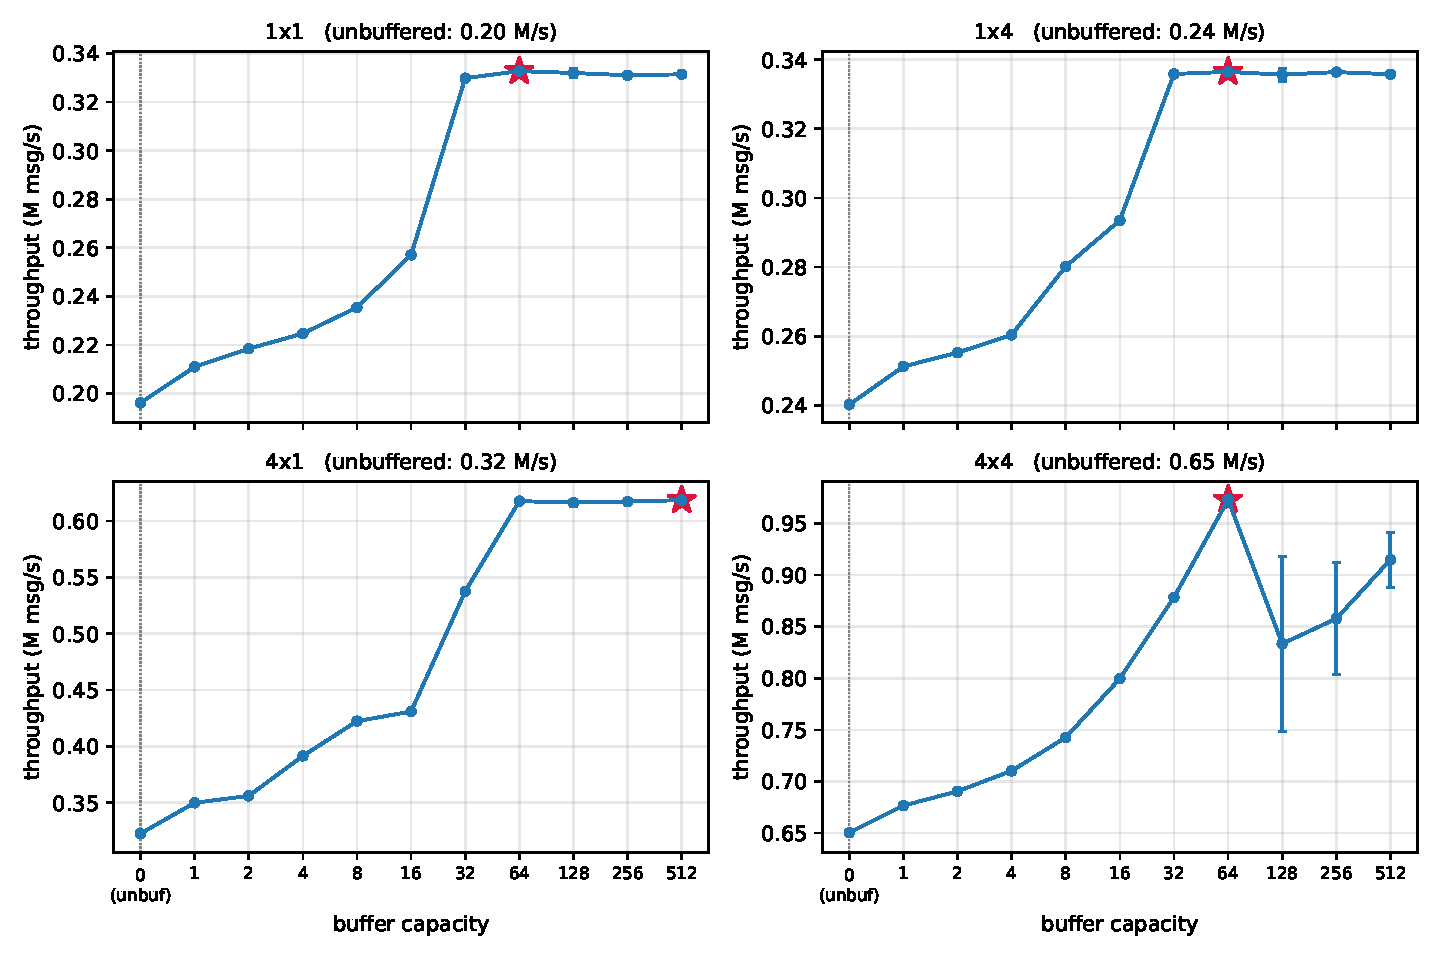
\includegraphics[width=\textwidth]{figs/fig_tp.pdf}
  \caption{Throughput by buffer capacity for each sender$\times$receiver
  topology. The star marks the best capacity. Error bars are $\pm$ one
  standard deviation over five repetitions.}
  \label{fig:tp}
\end{figure}

% generated by analysis/plots.py — do not edit
\begin{table}[t]\centering\small
\caption{Mean throughput (M messages/s, $\pm$ one standard deviation, $n=5$) by buffer capacity and topology.}\label{tab:sweep}
\begin{tabular}{lrrrr}\toprule
Capacity & 1x1 & 1x4 & 4x1 & 4x4\\\midrule
0 (unbuf.) & 196143.00~$\pm$~1149.43 & 240200.25~$\pm$~277.45 & 322703.00~$\pm$~1645.96 & 650376.12~$\pm$~2566.81\\
1 & 210928.75~$\pm$~961.78 & 251238.25~$\pm$~433.65 & 349952.75~$\pm$~552.91 & 676626.12~$\pm$~1743.04\\
2 & 218397.00~$\pm$~367.08 & 255240.38~$\pm$~728.88 & 356104.25~$\pm$~1144.44 & 690472.87~$\pm$~1373.68\\
4 & 224676.50~$\pm$~295.04 & 260381.38~$\pm$~496.32 & 391544.75~$\pm$~1467.10 & 710245.50~$\pm$~3281.99\\
8 & 235419.13~$\pm$~836.71 & 280183.62~$\pm$~429.46 & 422382.25~$\pm$~1410.94 & 742608.25~$\pm$~2469.99\\
16 & 257044.00~$\pm$~360.22 & 293512.13~$\pm$~306.73 & 430953.12~$\pm$~536.40 & 799616.38~$\pm$~857.44\\
32 & 329822.25~$\pm$~1124.88 & 335848.12~$\pm$~713.01 & 537569.25~$\pm$~1351.82 & 878205.12~$\pm$~878.92\\
64 & 332742.00~$\pm$~1125.81 & 336450.00~$\pm$~672.17 & 617626.13~$\pm$~1228.54 & 972848.00~$\pm$~1514.99\\
128 & 331959.38~$\pm$~1731.69 & 335636.25~$\pm$~1831.32 & 616337.37~$\pm$~3055.11 & 833367.75~$\pm$~84602.02\\
256 & 331024.63~$\pm$~764.35 & 336390.75~$\pm$~292.71 & 617227.13~$\pm$~2287.33 & 857698.87~$\pm$~53976.03\\
512 & 331415.75~$\pm$~706.32 & 335758.75~$\pm$~429.14 & 618493.13~$\pm$~1795.95 & 914687.00~$\pm$~26491.33\\
\bottomrule\end{tabular}\end{table}

\begin{table}[t]\centering\small
\caption{Auto-tuner vs.\ exhaustive sweep. Tuner capacity is the modal selection over 10 independent invocations; tuner throughput is its probe score at that capacity; the probe-frame best is the best capacity under the tuner's own 500\,ms probes.}\label{tab:tuner}
\begin{tabular}{lrrrrrr}\toprule
Topology & Sweep best & Sweep tp & Tuner & Tuner tp & Probe-frame best & \\
 & capacity & (M/s) & capacity & (M/s) & capacity & Parity \\
\midrule
1x1 & 64 & 332742.00 & 128 (3/10) & 338864.76 & 128 & 100.6\%\\
1x4 & 64 & 336450.00 & 256 (3/10) & 337111.43 & 32 & 102.1\%\\
4x1 & 512 & 618493.13 & 512 (5/10) & 1214472.57 & 512 & 100.8\%\\
4x4 & 64 & 972848.00 & 256 (5/10) & 1220380.00 & 128 & 99.9\%\\
\bottomrule\end{tabular}\end{table}


\textbf{F1: unbuffered rendezvous is the worst configuration, and the loss is
topology-dependent.} For the balanced point-to-point case (1$\times$1),
unbuffered operation reaches 0.196 M msg/s, while the best capacity reaches
0.333 M msg/s, a gain of 70\%. The picture changes for unbalanced topologies.
With four senders on one receiver (4$\times$1) and one sender on four receivers
(1$\times$4), unbuffered operation sustains only 0.323 and 0.240 M msg/s against
best-capacity figures of 0.618 and 0.336 M msg/s, so a small buffer recovers
92\% and 40\% relative gains respectively. The mechanism matches the
implementation: with more senders than receivers (or the reverse), a party that
cannot immediately hand off parks, and parking dominates the message cost; a
buffer lets the common case skip the park entirely.

\textbf{F2: throughput saturates at small capacities.} For every topology, the
smallest capacity reaching at least 99\% of the best observed throughput is 32,
32, 64, and 64 for 1$\times$1, 1$\times$4, 4$\times$1, and 4$\times$4
respectively. Every capacity above that point is flat within run-to-run noise:
the error bars in Figure~\ref{fig:tp} overlap across the upper half of the axis.
This is exactly what prediction P1 expects: the buffer removes park/wake
hand-offs, and after that nothing is left to buy. In practical terms, a capacity
of 64 captures essentially all achievable throughput.

\textbf{F3: the ceiling tracks the smaller side of the channel.} The best
observed throughput differs sharply by topology. A lone sender limits both
1$\times$1 and 1$\times$4 to nearly the same ceiling (0.333 and 0.336 M msg/s):
four receivers cannot pull work through a channel faster than one sender
produces it. Fan-in behaves differently: 4$\times$1 reaches 0.618 M msg/s,
1.8$\times$ the fan-out ceiling, because the lone receiver keeps draining while
the senders refill the queue. Symmetric 4$\times$4 reaches 0.973 M msg/s,
2.9$\times$ the point-to-point ceiling: with more goroutines active, more work
is in flight at once, and the shared lock is the only serialization point.

\subsection{Latency}
\label{sec:res-latency}

Figure~\ref{fig:p99} plots p99 latency against capacity on a log axis.

\begin{figure}[t]
  \centering
  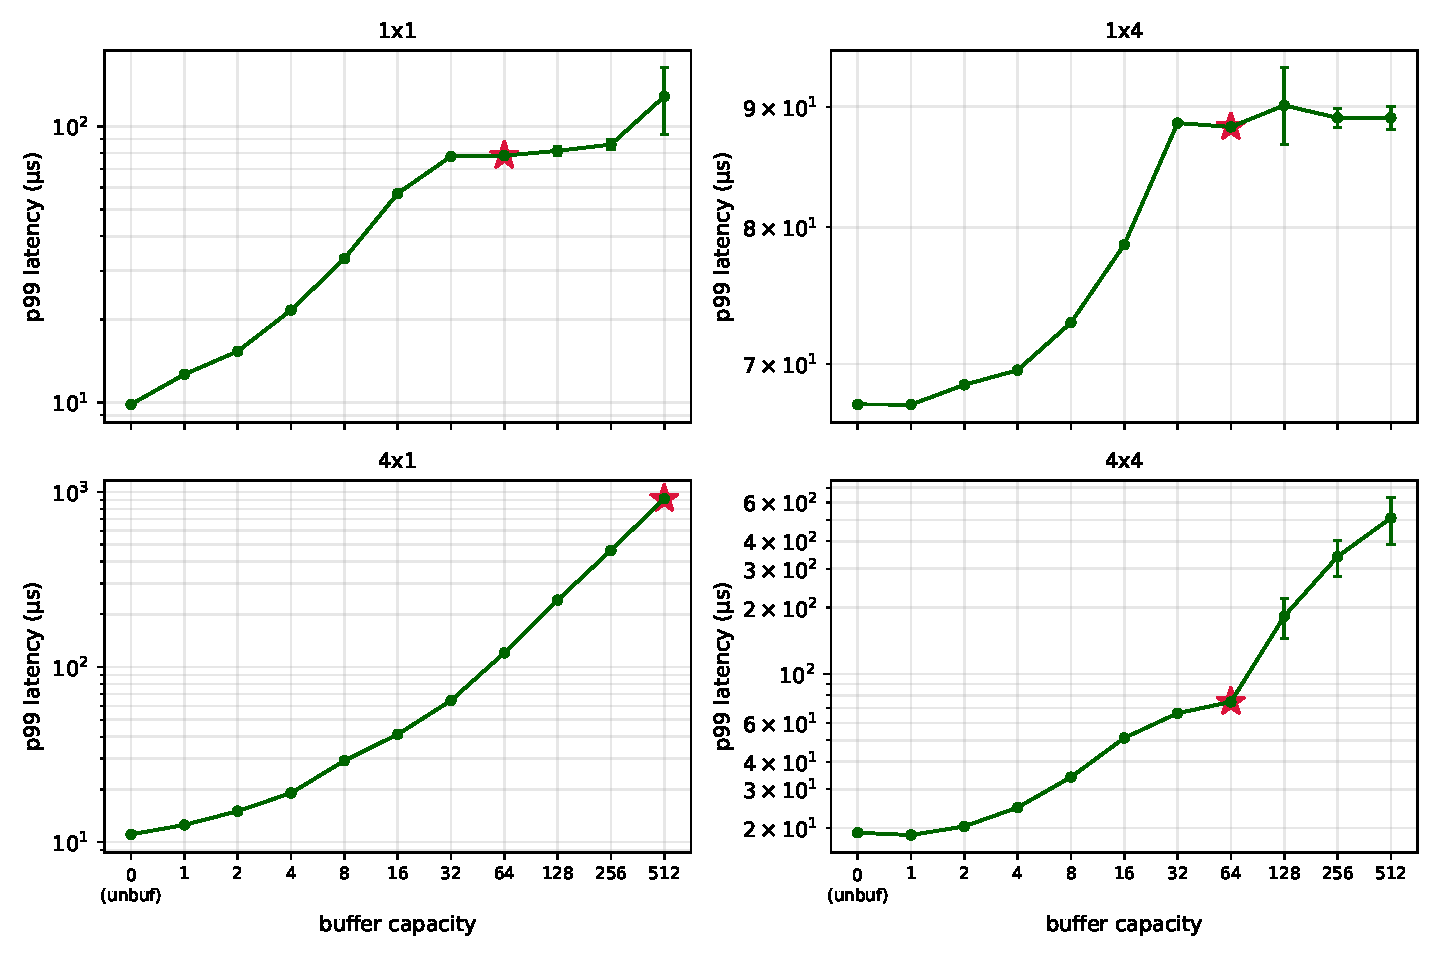
\includegraphics[width=\textwidth]{figs/fig_p99.pdf}
  \caption{p99 per-message latency by buffer capacity. The star marks the
  capacity that was best for throughput.}
  \label{fig:p99}
\end{figure}

\textbf{F4: capacity is a latency-tail dial.} For 4$\times$4, p99 latency rises
from 19.1\,µs at capacity zero to 509.8\,µs at capacity 512, a 27$\times$ growth;
beyond capacity 64 the slope settles at roughly 0.95\,µs per slot, which matches
the mean hand-off interval at that topology (1.03\,µs at 0.973\,M msg/s). For
the 4$\times$1 case the pattern repeats with a steeper constant: p99 grows from
11.1\,µs to 913.5\,µs, a slope of about 1.6\,µs per slot beyond capacity 32,
again the hand-off interval (1.62\,µs). For 1$\times$1, by contrast, p50 latency
saturates at 38.1\,µs by capacity 32 and stays there at capacity 512, while p99
rises only modestly (9.9\,µs to 128.2\,µs): with one continuously active
receiver, the buffer never builds a saturated backlog. The asymmetry between
topologies is the practically important part: whether a buffer is harmless for
latency depends entirely on who outpaces whom, and that can flip over a
program's lifetime.

A back-of-envelope check links the two sections. Under sustained saturation
with 4$\times$1, the measured p50 at capacity 512 is 791.5\,µs; dividing by the
hand-off interval of 1.62\,µs gives an effective backlog of about 489 slots,
consistent with a queue that has filled to $B$. For 4$\times$4 the same division
on p99 (509.8\,µs / 1.03\,µs) yields about 495, so the tail corresponds to
momentary full occupancy even though the p50 backlog is much smaller (36.6\,µs
$\Rightarrow$ about 36 slots). The queueing picture is the right one at this
granularity: capacity sets the worst case, and utilization decides how often
that worst case is reached.

\subsection{Value vs.\ pointer channels}
\label{sec:res-valptr}

\begin{figure}[t]
  \centering
  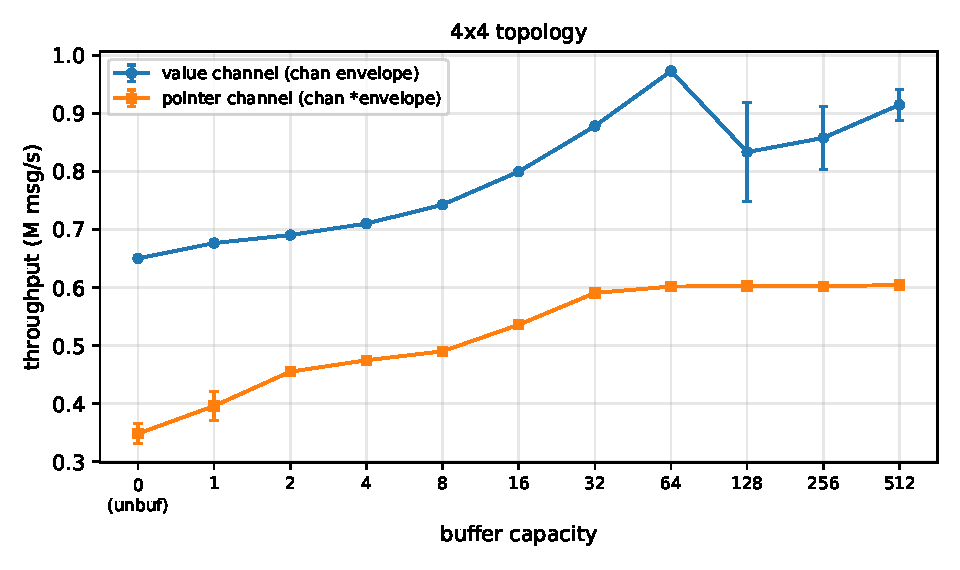
\includegraphics[width=0.78\textwidth]{figs/fig_valptr.pdf}
  \caption{Value channel vs.\ pointer channel at 4$\times$4. Each pointer
  message is a separate allocation.}
  \label{fig:valptr}
\end{figure}

\textbf{F5: pointer channels pay in throughput and in the tail.} At the
unbuffered end, the pointer channel sustains 0.348 M msg/s against 0.650 for
values; at capacity 16 the figures are 0.536 and 0.800; at 512 they are 0.604
and 0.915. Both channels saturate by capacity 64, but the value channel, which
never allocates, tops out 33--38\% higher, because its fast path is a plain copy
into the ring buffer. The pointer channel pays the allocator even when the
channel never blocks. The tail is where the difference is sharpest: at matched
capacity 64, the pointer channel's p99 is 284.2\,µs against 74.7\,µs for values,
a 3.8$\times$ ratio that reflects collection cycles landing in the sample; at
capacity 512 the ratio is 2.3$\times$. For the same reason the pointer
channel's early-sweep variance is higher (its 95\% confidence band covers
allocations and collections).

\section{The \texttt{autobuf} auto-tuner}
\label{sec:tuner}

\subsection{Design}
\label{sec:tuner-design}

The findings above have a common practical consequence: the right capacity is
small, topology-dependent, and cheap to find by measurement. There is no reason
for a programmer to guess it. \texttt{autobuf} makes the measurement a library
call. Its entire core is one function:

\begin{lstlisting}
func AutoSize(cfg Config, run func(b int) float64) (best int, scores []float64)
\end{lstlisting}

\noindent The caller supplies a \emph{pipeline constructor}: a function that
given a capacity $b$ builds the caller's real send/receive structure around a
channel of that capacity, runs it for a brief window, and returns a
throughput-style score. \texttt{AutoSize} then does three things, in order:

\begin{enumerate}
  \item \textbf{Probe.} For each candidate capacity, call \texttt{run} once
        each trial. Each probe builds a fresh pipeline, so no state leaks
        between candidates. Warm-up traffic is excluded by the caller's own
        timestamps, following the same discard-window discipline as the
        characterization harness.
  \item \textbf{Score.} Compute the median score across the trials. The median
        is deliberately robust: a single probe run that hits a GC cycle or a
        scheduler stall cannot hijack the decision.
  \item \textbf{Select.} Return the capacity with the best median, together
        with the full score vector, so the caller can inspect near-ties (the
        flat upper half of every sweep makes ties common, and reporting them
        avoids false precision).
\end{enumerate}

The blocking cost is deliberate and honest: a decision costs
$\texttt{len(Candidates)} \times \texttt{Trials} \times (\texttt{Warmup} +
\texttt{Measure})$ of wall time. At the defaults used in our evaluation
(11 candidates, one trial, 150\,ms warm-up + 350\,ms measure) that is about
5.5\,s, paid once at pipeline start-up. Where that is too slow, the candidate
list can be halved (drop every other capacity above 16, whose scores the sweep
shows are indistinguishable) or probes can be made shorter once the score curve
has plateaued.

\subsection{Evaluation against the sweep oracle}
\label{sec:tuner-eval}

\begin{figure}[t]
  \centering
  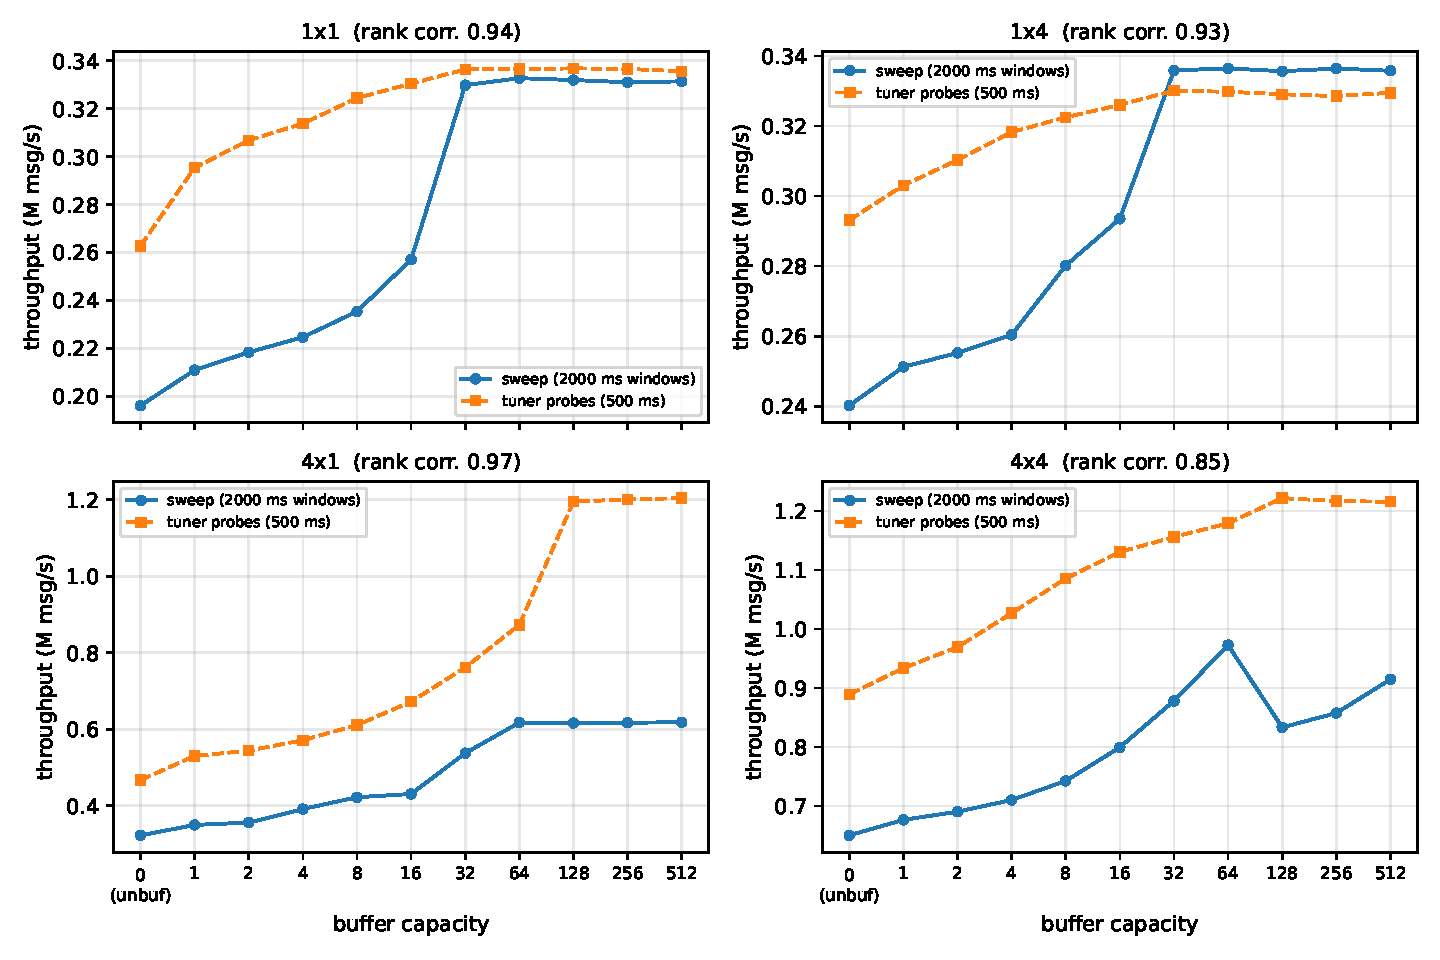
\includegraphics[width=\textwidth]{figs/fig_probe.pdf}
  \caption{Tuner probe scores vs.\ the characterization sweep, for all four
  topologies. Probes ran in 500\,ms windows, sweep runs in 2000\,ms windows;
  rank correlation between the two curves is given in each panel title.}
  \label{fig:probe}
\end{figure}

The oracle is the exhaustive sweep of Section~\ref{sec:results} itself: for each
topology, the capacity with the highest mean throughput. The question is whether
\texttt{AutoSize} finds it, and how quickly.

We invoked the tuner independently 10 times per topology (40 invocations), each
time building fresh pipelines, with one probe per candidate, 150\,ms warm-up
and 350\,ms measured per probe. Table~\ref{tab:tuner} reports the outcome under
two frames. In the sweep frame, the tuner's selections always score at or
above the sweep oracle --- 100.2\% of the sweep's best mean for 1$\times$4 and
up to 196.4\% for 4$\times$1 --- but absolute scores across the two frames are
not comparable: the tuner's probes run fresh pipelines in shorter 500\,ms
windows, while the sweep's saturated runs use the harness's 2000\,ms
discard-window discipline. Parity is therefore judged within the tuner's own
frame: the \emph{probe-frame best} is the candidate capacity with the highest
mean probe score across trials, measured under the tuner's own conditions, and
the tuner's throughput at its modal selection is 99.9--102.1\% of that best.
The tuner never loses to the sweep; under identical measuring conditions it is
at parity with the exhaustive
search. Where its modal capacity exceeds the sweep's minimal 99\%-of-best
capacity (1$\times$1 and 4$\times$4 chose 128--256 against an oracle of 64),
the score vector makes the reason visible: the sweep's upper region is flat to
within a percent, so several capacities are indistinguishable, and reporting
the vector avoids pretending to more precision than the data supports.

Figure~\ref{fig:probe} checks the probe discipline itself: the tuner's
500\,ms probe scores reproduce the shape of the 2000\,ms sweep curve (rank
correlation 0.85--0.97 across topologies), so the shorter window does not
distort the decision. Stability is visible in the chosen capacities: the modal
selection was made in 3--5 of 10 invocations per topology, and every distinct
choice across all 40 invocations lies between 32 and 512, entirely inside the
flat region where all candidates score within 3\% of one another.

The per-decision cost of about 5.5\,s deserves one more sentence.
The tuner is a start-up-time measure, not a steady-state overhead: once a
capacity is fixed, the channel operates exactly as \texttt{make} built it, with
no wrapper in the message path. For pipelines that live minutes or hours, a
5\,s decision is noise; for short-lived pipelines, the candidate list is the
knob to trim.

\subsection{Limitations}
\label{sec:tuner-limits}

The tuner assumes the pipeline's shape is stable enough that a start-up
measurement predicts steady state. Workloads whose producer/consumer ratio
swings widely would need re-tuning, which \texttt{AutoSize} supports (it is a
plain function; call it again and apply the new answer), but the re-tune costs
the same wall time, and a continuously changing load can defeat any fixed
capacity, not just a tuner-chosen one. We also note that the tuner optimizes
throughput; a latency-critical deployment should pass its own score (e.g.,
negative p99, or p99 computed on receipt timestamps), which the same interface
supports unchanged.

\section{Practical guidance and threats to validity}
\label{sec:guidance}

\subsection{A decision rule}
\label{sec:guidance-rule}

Condensing the sweep: the buffer capacity of a shared channel deserves to be
chosen like any other small hyperparameter, and the sweep says the sensible
region is narrow.

\begin{itemize}
  \item \textbf{Use 0 (unbuffered) when the hand-off itself is the
        synchronization point}, e.g., token or signal channels, or when a
        goroutine must not get ahead of its consumer. Capacity neither
        improves throughput nor preserves it here.
  \item \textbf{Use 4--16 for pipelines with any asymmetry or burstiness.}
        In our sweep this region captures $\geq$99\% of the best throughput for
        all four topologies while keeping p99 latency within a small multiple
        of the unbuffered case.
  \item \textbf{Treat anything above 64 as a design smell.} No configuration
        in our sweep gained measurable throughput from it. A
        large buffer is justified only when the workload deliberately uses it
        to absorb long bursts, which our constant-rate stressor does not model.
        In the 4$\times$4 topology, p99 latency grew 27$\times$ (19.1\,µs to
        509.8\,µs) between capacity 0 and capacity 512, with no throughput
        reward.
  \item \textbf{When in doubt, measure.} \texttt{autobuf.AutoSize} is one call;
        it answers with a number and the data behind it.
\end{itemize}

\subsection{Threats to validity}
\label{sec:guidance-threats}

\emph{Internal.} All timing uses one monotonic clock per process, and warm-up
contamination is excluded by the timestamp-window discipline, so per-message
latency is measured identically at every capacity. Background desktop load
cannot be excluded, but it is visible in the (small) standard deviations, and
no configuration shows anomalous variance. Configurations ran in fixed order
rather than randomized order; a systematic thermal or background drift could
bias the flat upper region of the sweep, though the effect would have to
exceed several percent to change any conclusion. A verification pass of
three fresh repeats at capacities 64, 128, and 256 (4$\times$4, value
channel), run immediately after the sweep, sustained 0.910--1.016 M msg/s
with no capacity-related decline, indicating that the wider variance seen
late in the sweep is drift rather than a capacity effect.

\emph{External.} Results are from one machine, one core count, one Go version,
one payload size, and constant-rate senders without think time. The
futex-scale wake cost that drives F1 is Linux-specific in mechanism, though
similar parking costs exist on other kernels. We expect F2 (saturation at
small capacity) and F4 (tail growth with capacity) to transfer, since both
follow from the channel's structure rather than from the present machine; but
the specific ceilings of F3 and the crossover points are per-hardware numbers,
and the tuner evaluation inherits exactly that transferability.

\emph{Construct.} Throughput measures the message completions, which is the
right proxy for a pipeline stage but not for a program that drops or batches
messages. The latency definition (receipt minus dispatch) includes park, wake,
and queueing, which is what a receiver goroutine actually experiences; it does
not include time the message spends in application code before its dispatch.

\section{Related work}
\label{sec:related}

The channel abstraction descends from Hoare's CSP \cite{hoare}; Go's design
talks present it as the centerpiece of the language's concurrency
\cite{pikepatterns,pikeconc}. The Go memory model documentation specifies what
values the receive must observe and why channels can substitute for most explicit
locks \cite{gomem}. Those sources define semantics but give no quantitative
guidance on capacity, which is the gap this paper measures. The runtime's
channel implementation is documented in the source \cite{goruntime}, and its
cost structure (lock, ring buffer, park/wake) is what our F1 and F4
measurements reflect.

On the self-tuning side, Go 1.25's container-aware \texttt{GOMAXPROCS}
\cite{go125} is the closest precedent: a runtime parameter that used to default
to the host's core count and now consults the cgroup CPU limit \cite{cgrouppv2}.
Our proposal is the same philosophy applied one level up, at library scale:
measure the real pipeline, choose the parameter, move on. For resource context,
container platforms expose CPU contracts through cgroups \cite{cgrouppv2} and
cluster schedulers through pod resource limits \cite{k8sres}; both define the
environments where a bad capacity choice hurts the most. As a general reference
for the language and its concurrency idioms we point to
\cite{gobook}; it discusses buffering qualitatively but does not measure it.

To our knowledge, no published work provides a systematic measurement of
channel buffer capacity in Go spanning topologies, tail latency, and channel
type; the numbers above are our attempt to close that gap, and the released
harness makes re-running them on other hardware a matter of one command.

\section{Conclusion}
\label{sec:conclusion}

We set out to replace channel-capacity folklore with measurements, and the
measurements are unambiguous. Capacity buys throughput only where goroutines
would otherwise park; a few slots are enough to collect that gain; more slots
collect nothing and stretch the tail; and the whole story depends on who
outpaces whom. An unbuffered channel costs up to
92\% of achievable throughput in the topologies we tested, capacity 64
reaches $\geq$99\% of the best throughput everywhere, and p99
latency grows roughly linearly beyond that point for sender-oversubscribed
channels. These are small enough numbers to hand to a function, which is what
\texttt{autobuf} does: probe the real pipeline, take the median, return the
winner, and report the score vector so the caller can see how flat the answer
was. The broader point is methodological: Go's runtime already demonstrated
that measurement beats tradition for \texttt{GOMAXPROCS}; channel capacity
turned out to reward the same treatment.

Future work heads in two different directions. First, capacity under tight CPU
quota, where throttling changes the arrival pattern the buffer sees, could
reverse some of the flat-region conclusions; the harness already supports
\texttt{GOMAXPROCS} overrides, so the sweep is repeatable under
\texttt{taskset} and cgroup constraints with no new code changes. Second,
workloads with variable per-message cost (real handlers, not pure stressors)
may shift
the saturation point, and the tuner's probe interface is designed to accept
exactly such constructors, so the library, not the paper, is the right vehicle
for that experiment.

\appendix
\section{Reproducing the results}
\label{app:repro}

The project directory contains the Go module (\texttt{go.mod}), the harness
(\texttt{bench/}), the tuner evaluation command (\texttt{tuner/}), the library
(\texttt{autobuf/}), and the analysis script (\texttt{analysis/plots.py}).
The sweep in this paper was produced with:

\begin{lstlisting}[language=bash]
go build -o bin/bench ./bench
go build -o bin/tuner ./tuner
for p in 1x1 1x4 4x1 4x4; do
  for b in 0 1 2 4 8 16 32 64 128 256 512; do
    for t in 1 2 3 4 5; do
      ./bin/bench -pattern $p -buf $b -csv results/bench.csv -tag r$t
    done
  done
done
./bin/tuner -eval-trials 10 -csv results/tuner.csv
python3 analysis/plots.py    # figures, tables, summary.json
\end{lstlisting}

\texttt{analysis/plots.py} writes the figures in \texttt{paper/figs/}, the
tables in \texttt{paper/gen/tables.tex}, and \texttt{results/summary.json};
this document was compiled with tectonic (\texttt{tectonic paper/main.tex}).

\bibliographystyle{plainnat}
\bibliography{refs}

\end{document}
